\documentclass[bachelor, och, labwork]{SCWorks}
% параметр - тип обучения - одно из значений:
%    spec     - специальность
%    bachelor - бакалавриат (по умолчанию)
%    master   - магистратура
% параметр - форма обучения - одно из значений:
%    och   - очное (по умолчанию)
%    zaoch - заочное
% параметр - тип работы - одно из значений:
%    referat    - реферат
%    coursework - курсовая работа (по умолчанию)
%    diploma    - дипломная работа
%    pract      - отчет по практике
% параметр - включение шрифта
%    times    - включение шрифта Times New Roman (если установлен)
%               по умолчанию выключен
\usepackage{subfigure}
\usepackage{tikz,pgfplots}
\pgfplotsset{compat=1.5}
\usepackage{float}

%\usepackage{titlesec}
\setcounter{secnumdepth}{4}
%\titleformat{\paragraph}
%{\normalfont\normalsize}{\theparagraph}{1em}{}
%\titlespacing*{\paragraph}
%{35.5pt}{3.25ex plus 1ex minus .2ex}{1.5ex plus .2ex}

\titleformat{\paragraph}[block]
{\hspace{1.25cm}\normalfont}
{\theparagraph}{1ex}{}
\titlespacing{\paragraph}
{0cm}{2ex plus 1ex minus .2ex}{.4ex plus.2ex}

% --------------------------------------------------------------------------%
\usepackage[T2A]{fontenc}
\usepackage[utf8]{inputenc}
\usepackage{graphicx}
\graphicspath{ {./img/} }
\usepackage{tempora}

\usepackage[sort,compress]{cite}
\usepackage{amsmath}
\usepackage{amssymb}
\usepackage{amsthm}
\usepackage{fancyvrb}
\usepackage{listings}
\usepackage{listingsutf8}
\usepackage{longtable}
\usepackage{array}
\usepackage[english,russian]{babel}

\usepackage[colorlinks=true, linkcolor=black]{hyperref}
\usepackage{url}

\usepackage{underscore}
\usepackage{setspace}
\usepackage{indentfirst} 
\usepackage{mathtools}
\usepackage{amsfonts}
\usepackage{enumitem}
\usepackage{tikz}

\usepackage{minted}
\setminted[python3]{style=bw, linenos, breaklines=true, fontsize=\footnotesize}

\newcommand{\eqdef}{\stackrel {\rm def}{=}}
\newcommand{\specialcell}[2][c]{%
\begin{tabular}[#1]{@{}c@{}}#2\end{tabular}}

\renewcommand\theFancyVerbLine{\small\arabic{FancyVerbLine}}

\newtheorem{lem}{Лемма}

\begin{document}

% Кафедра (в родительном падеже)
\chair{теоретических основ компьютерной безопасности и криптографии}

% Тема работы
\title{Теория псевдослучайных генераторов}

% Курс
\course{4}

% Группа
\group{431}

% Факультет (в родительном падеже) (по умолчанию "факультета КНиИТ")
\department{факультета КНиИТ}

% Специальность/направление код - наименование
%\napravlenie{09.03.04 "--- Программная инженерия}
%\napravlenie{010500 "--- Математическое обеспечение и администрирование информационных систем}
%\napravlenie{230100 "--- Информатика и вычислительная техника}
%\napravlenie{231000 "--- Программная инженерия}
\napravlenie{10.05.01 "--- Компьютерная безопасность}

% Для студентки. Для работы студента следующая команда не нужна.
% \studenttitle{Студентки}

% Фамилия, имя, отчество в родительном падеже
\author{Стаина Романа Игоревича}

% Заведующий кафедрой
\chtitle{} % степень, звание
\chname{}

%Научный руководитель (для реферата преподаватель проверяющий работу)
\satitle{доцент} %должность, степень, звание
\saname{И.~И.~Слеповичев}

% Руководитель практики от организации (только для практики,
% для остальных типов работ не используется)
% \patitle{к.ф.-м.н.}
% \paname{С.~В.~Миронов}

% Семестр (только для практики, для остальных
% типов работ не используется)
%\term{8}

% Наименование практики (только для практики, для остальных
% типов работ не используется)
%\practtype{преддипломная}

% Продолжительность практики (количество недель) (только для практики,
% для остальных типов работ не используется)
%\duration{4}

% Даты начала и окончания практики (только для практики, для остальных
% типов работ не используется)
%\practStart{30.04.2019}
%\practFinish{27.05.2019}

% Год выполнения отчета
\date{2023}

\maketitle

% Включение нумерации рисунков, формул и таблиц по разделам
% (по умолчанию - нумерация сквозная)
% (допускается оба вида нумерации)
% \secNumbering

%-------------------------------------------------------------------------------------------

% \begin{minted}[fontsize=\small]{MySQL}
% \end{minted}

% \begin{figure}[H]
%     \centering
%     \includegraphics[width=0.999\textwidth]{img/}
%     \caption{}
% \end{figure}

\tableofcontents

\section{Постановка задачи}
\textbf{Цель}.
\begin{enumerate}
  \item Сгенерировать псевдослучайную последовательность заданным методом. 
  \item Исследовать полученную псевдослучайную последовательность на случайность.
\end{enumerate}

\textbf{Исходные данные}. Исходными данными для лабораторных занятий являются метод генерации псевдослучайных чисел, 
диапазон генерации случайных чисел, функция распределения, которой должны подчиняться случайные 
числа, количество генерируемых чисел. 

В данной работе были исследованы ППСЧ длиной 10000 элементов по модулю 1024, реализованные в практической работе №1. Их входные переменные, передаваемые через параметр \texttt{/i}:
\begin{enumerate}
  \item Линейный конгруэнтный метод: \texttt{/i:31104,625,6571,23}.
  \item Аддитивный метод: {\footnotesize\texttt{/i:30000,24,55,79,134,213,347,560,907,1467,2374,3841,6215,\\10056,16271,26327,12598,8925,21523,448,21971,22419,14390,6809,21199,28008,19207,\\17215,6422,23637,59,23696,23755,17451,11206,28657,9863,8520,18383,26903,15286,12189,\\27475,9664,7139,16803,23942,10745,4687,15432,20119,5551,25670,1221,26891,28112,\\23779,17506}}.
  \item Пятипараметрический метод: {\footnotesize\texttt{/i:89,7,13,24,10,234122131}}.
  \item РСЛОС: {\footnotesize\texttt{/i:10011011010011010,17}}.
  \item Нелинейная комбинация РСЛОС: {\footnotesize\texttt{/i:00000001010101,01011100000111101,\\010101001100000,97,1234,345231,10}}.
  \item Вихрь Мерсенна: {\footnotesize\texttt{/i:1024,1234}}.
  \item RC4: {\footnotesize\texttt{/i:213,968,838,64,355,214,212,36,695,139,897,518,656,956,810,510,985,105,670,\\8,907,951,685,989,222,931,169,286,289,556,731,902,688,701,771,533,990,630,708,884,\\255,683,25,214,792,348,34,758,9,781,946,580,615,955,585,5,886,563,81,38,809,444,619,\\222,544,53,635,621,630,251,497,257,2,467,897,790,728,676,722,838,465,781,10,828,903,\\235,857,841,146,719,681,678,961,652,491,38,256,909,251,21,110,811,273,25,642,286,489,\\478,184,812,770,846,241,141,266,500,375,827,633,761,154,663,461,206,529,212,667,342,\\360,165,523,749,582,803,553,345,786,990,361,702,256,380,234,238,73,965,266,300,847,\\755,969,681,146,843,125,306,845,752,879,458,788,833,727,817,122,239,765,877,827,327,\\733,658,644,880,150,474,493,689,670,368,611,263,113,417,834,103,725,754,117,824,623,\\338,540,337,879,521,183,370,808,120,571,871,301,210,796,744,398,106,845,745,842,876,\\399,27,105,601,802,831,53,266,157,352,175,303,505,484,994,425,292,729,654,584,860,\\420,412,49,281,417,703,400,48,404,772,389,733,152,271,585,404,333,381,696,928,609,\\659,180}}.
  \item RSA: {\footnotesize\texttt{/i:10967,571,77,10}}.
  \item Блюм-Блюма-Шуба: {\footnotesize\texttt{/i:239,10}}.
\end{enumerate}

\section{Статистические свойства последовательности псевдослучайных чисел}
\subsection{Вычисление оценок для ППСЧ}
Относительные погрешности измерялись для выборки из 5000 элементов.
\subsubsection{Линейный конгруэнтный метод}
\begin{figure}[H]
    \centering
    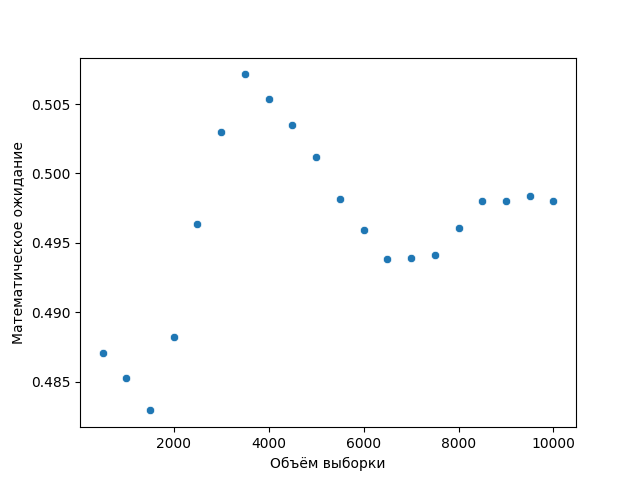
\includegraphics[width=0.63\textwidth]{lc_me.png}
    \caption{Зависимость математического ожидания от объёма выборки}
\end{figure}
Относительная погрешность измерения: 0.642\%.

\begin{figure}[H]
    \centering
    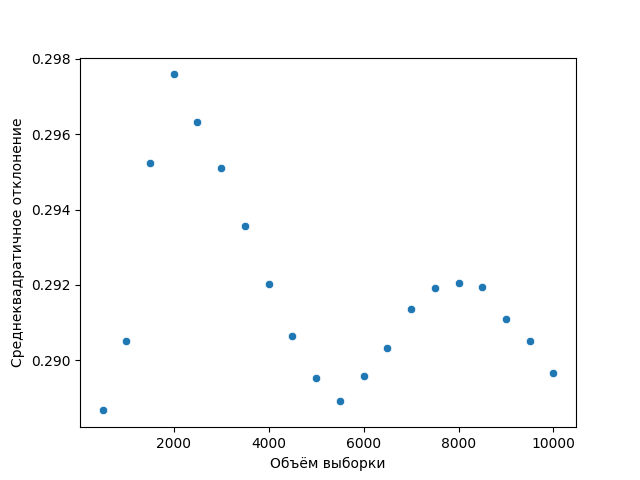
\includegraphics[width=0.63\textwidth]{lc_st.png}
    \caption{Зависимость среднеквадратичного отклонения от объёма выборки}
\end{figure}
Относительная погрешность измерения: 0.048\%.

\subsubsection{Аддитивный метод}
\begin{figure}[H]
  \centering
  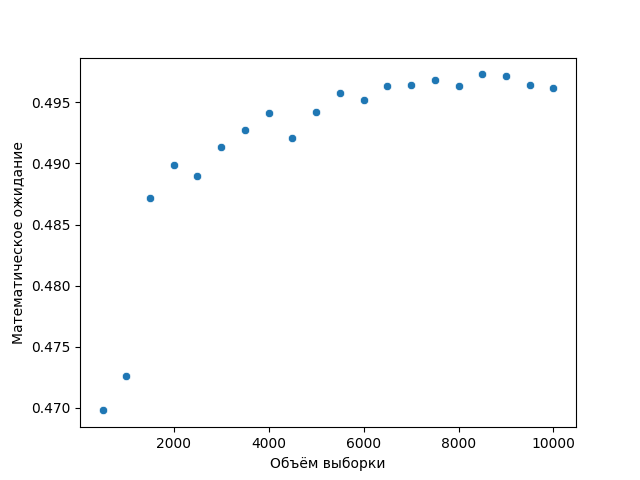
\includegraphics[width=0.7\textwidth]{add_me.png}
  \caption{Зависимость математического ожидания от объёма выборки}
\end{figure}
Относительная погрешность измерения: 0.4\%.

\begin{figure}[H]
  \centering
  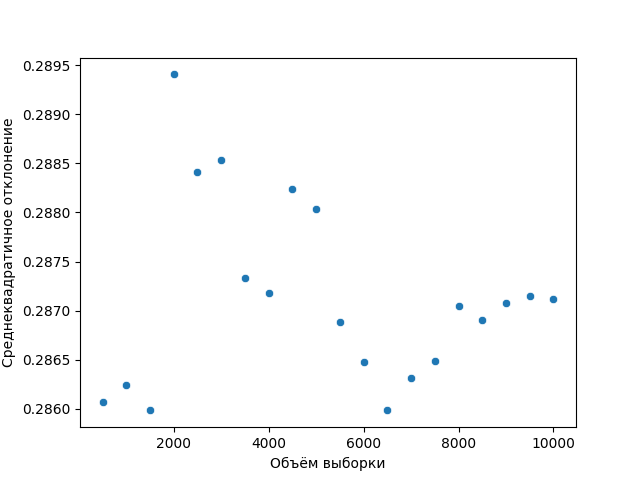
\includegraphics[width=0.7\textwidth]{add_st.png}
  \caption{Зависимость среднеквадратичного отклонения от объёма выборки}
\end{figure}
Относительная погрешность измерения: 0.316\%.

\subsubsection{Пятипараметрический метод}
\begin{figure}[H]
  \centering
  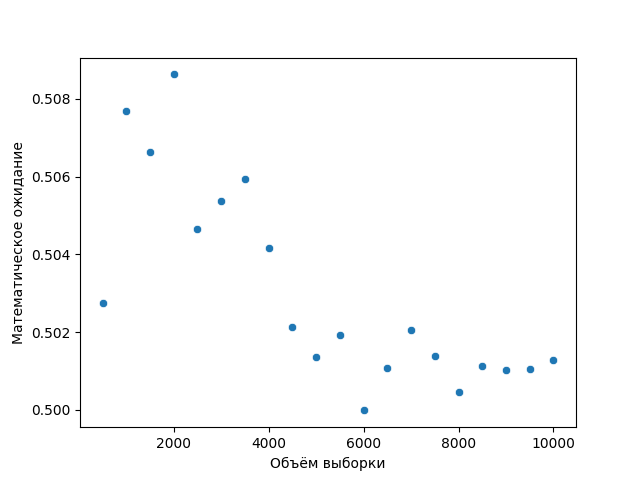
\includegraphics[width=0.7\textwidth]{5p_me.png}
  \caption{Зависимость математического ожидания от объёма выборки}
\end{figure}
Относительная погрешность измерения: 0.013\%.

\begin{figure}[H]
  \centering
  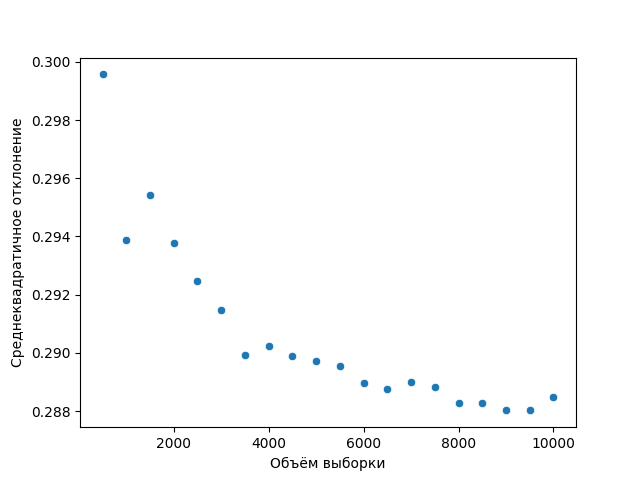
\includegraphics[width=0.7\textwidth]{5p_st.png}
  \caption{Зависимость среднеквадратичного отклонения от объёма выборки}
\end{figure}
Относительная погрешность измерения: 0.421\%.

\subsubsection{РСЛОС}
\begin{figure}[H]
  \centering
  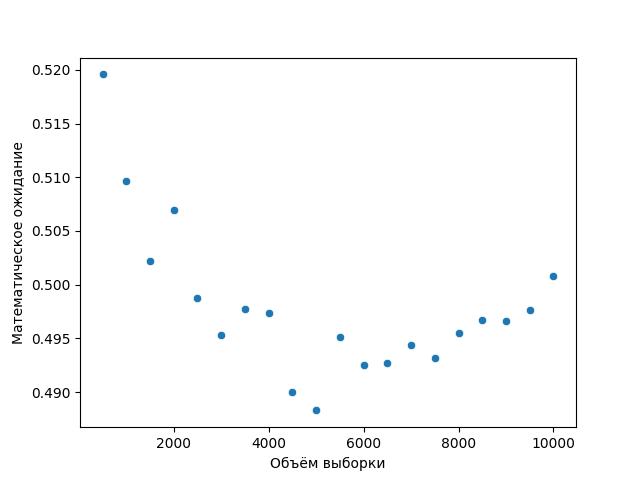
\includegraphics[width=0.7\textwidth]{lfsr_me.png}
  \caption{Зависимость математического ожидания от объёма выборки}
\end{figure}
Относительная погрешность измерения: 2.561\%.

\begin{figure}[H]
  \centering
  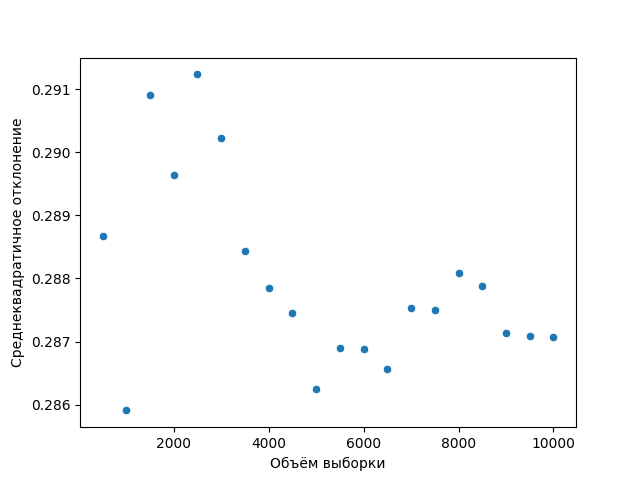
\includegraphics[width=0.7\textwidth]{lfsr_st.png}
  \caption{Зависимость среднеквадратичного отклонения от объёма выборки}
\end{figure}
Относительная погрешность измерения: 0.287\%.

\subsubsection{Нелинейная комбинация РСЛОС}
\begin{figure}[H]
  \centering
  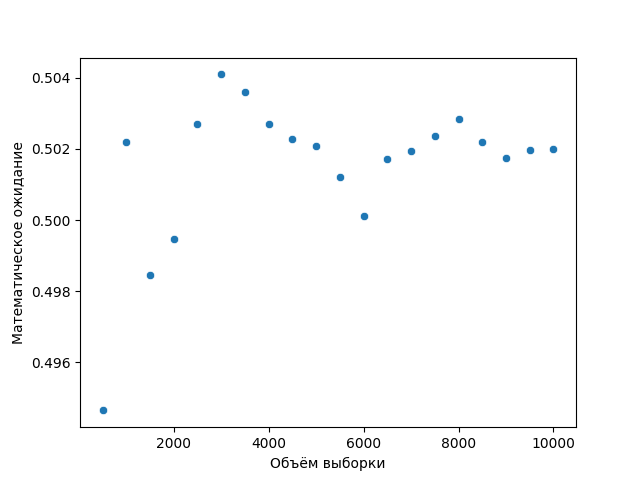
\includegraphics[width=0.7\textwidth]{nfsr_me.png}
  \caption{Зависимость математического ожидания от объёма выборки}
\end{figure}
Относительная погрешность измерения: 0.013\%.

\begin{figure}[H]
  \centering
  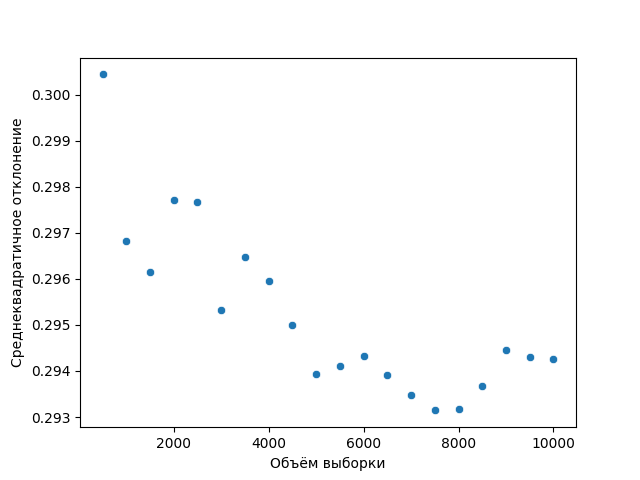
\includegraphics[width=0.7\textwidth]{nfsr_st.png}
  \caption{Зависимость среднеквадратичного отклонения от объёма выборки}
\end{figure}
Относительная погрешность измерения: 0.109\%.

\subsubsection{Вихрь Мерсенна}
\begin{figure}[H]
  \centering
  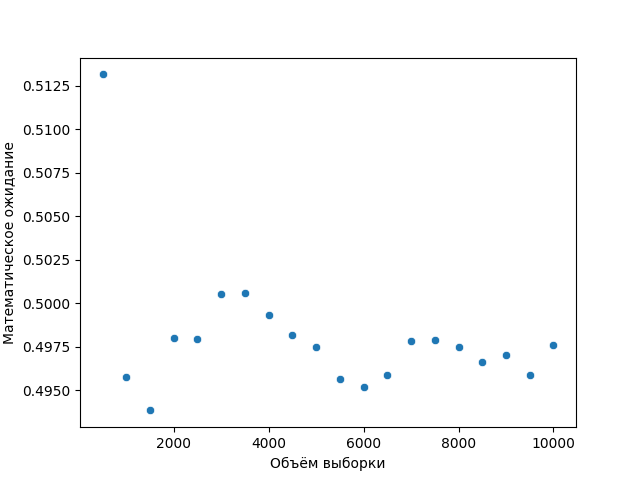
\includegraphics[width=0.7\textwidth]{mt_me.png}
  \caption{Зависимость математического ожидания от объёма выборки}
\end{figure}
Относительная погрешность измерения: 0.023\%.

\begin{figure}[H]
  \centering
  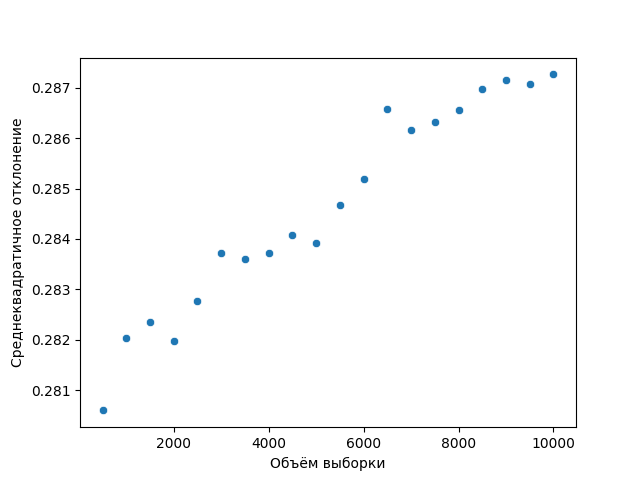
\includegraphics[width=0.7\textwidth]{mt_st.png}
  \caption{Зависимость среднеквадратичного отклонения от объёма выборки}
\end{figure}
Относительная погрешность измерения: 1.176\%.

\subsubsection{RC4}
\begin{figure}[H]
  \centering
  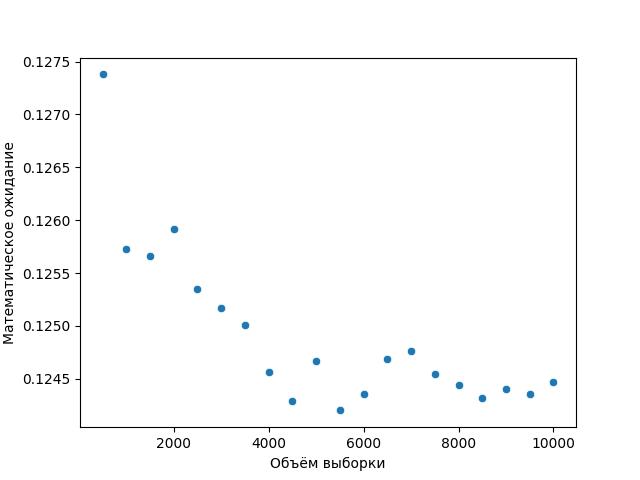
\includegraphics[width=0.7\textwidth]{rc_me.png}
  \caption{Зависимость математического ожидания от объёма выборки}
\end{figure}
Относительная погрешность измерения: 0.163\%.

\begin{figure}[H]
  \centering
  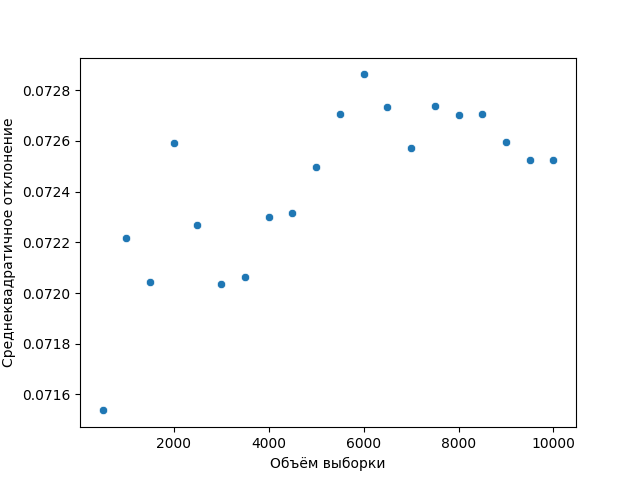
\includegraphics[width=0.7\textwidth]{rc_st.png}
  \caption{Зависимость среднеквадратичного отклонения от объёма выборки}
\end{figure}
Относительная погрешность измерения: 0.038\%.

\subsubsection{RSA}
\begin{figure}[H]
  \centering
  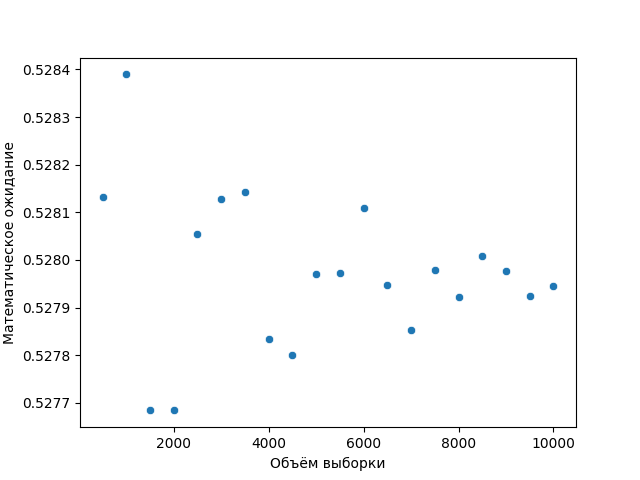
\includegraphics[width=0.7\textwidth]{rsa_me.png}
  \caption{Зависимость математического ожидания от объёма выборки}
\end{figure}
Относительная погрешность измерения: 0.005\%.

\begin{figure}[H]
  \centering
  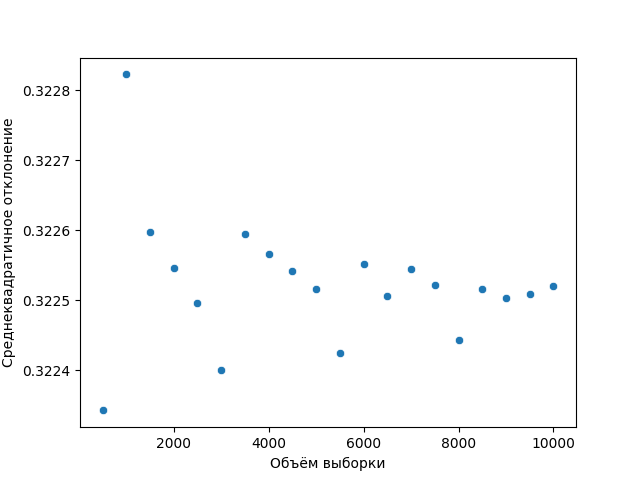
\includegraphics[width=0.7\textwidth]{rsa_st.png}
  \caption{Зависимость среднеквадратичного отклонения от объёма выборки}
\end{figure}
Относительная погрешность измерения: 0.001\%.

\subsubsection{Блюм-Блюма-Шуба}
\begin{figure}[H]
  \centering
  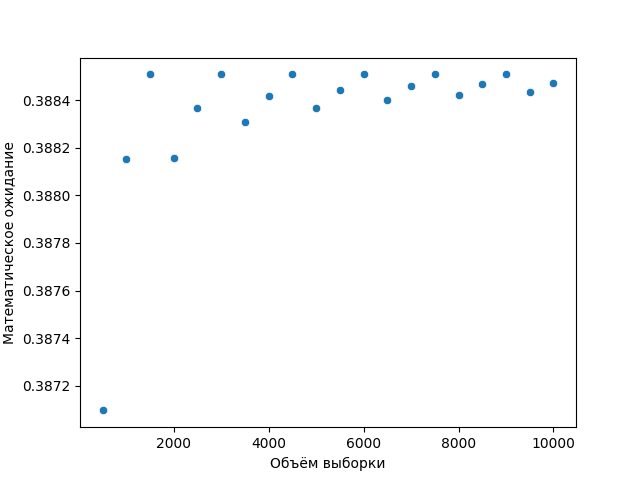
\includegraphics[width=0.7\textwidth]{bbs_me.png}
  \caption{Зависимость математического ожидания от объёма выборки}
\end{figure}
Относительная погрешность измерения: 0.027\%.

\begin{figure}[H]
  \centering
  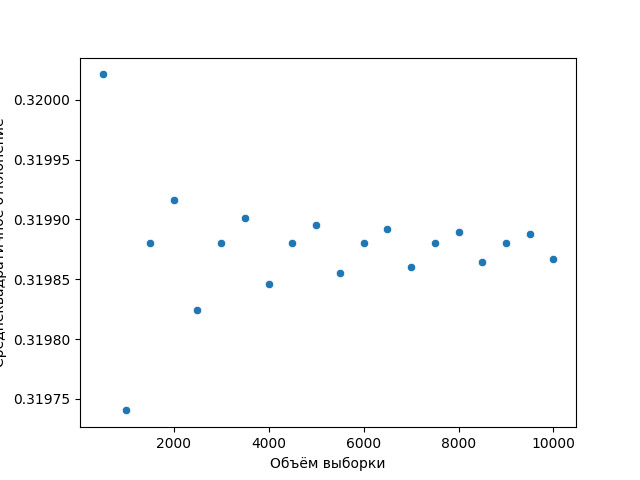
\includegraphics[width=0.7\textwidth]{bbs_st.png}
  \caption{Зависимость среднеквадратичного отклонения от объёма выборки}
\end{figure}
Относительная погрешность измерения: 0.009\%.

\subsection{Результаты проверок критериев ПСЧ}
\begin{table}[H]
  \resizebox{\textwidth}{!}{%
  \begin{tabular}{|l|l|l|l|l|l|l|l|}
  \hline
   & Хи-квадрат & Серий & Интервалов & Разбиений & Перестановок & Монотонности \\ \hline
  lc   & + & - & + & + & - & + \\ \hline
  add  & + & + & - & + & + & + \\ \hline
  5p   & + & + & + & + & + & -  \\ \hline
  lfsr & + & - & + & - & - & -  \\ \hline
  nfsr & - & - & - & - & + & + \\ \hline
  mt   & + & + & + & + & + & +  \\ \hline
  rc4  & + & + & + & + & + & +  \\ \hline
  rsa  & - & - & - & - & - & -  \\ \hline
  bbs  & + & - & - & - & - & -  \\ \hline
  \end{tabular}%
  }
\end{table}


% \begin{minted}[fontsize=\footnotesize]{python3}
% \end{minted}

\newpage
\appendix
    \section{Код \texttt{main.py}}
    \inputminted[fontsize=\footnotesize]{python3}{D:/CSIT/TPRG/LabWork/code/main.py}

%     \section{Код \texttt{Bit.py}}
%     \inputminted[fontsize=\footnotesize]{text}{code/Bit.py}

%     \section{Код \texttt{HuffmanEncode.py}}
%     \inputminted[fontsize=\footnotesize]{text}{code/HuffmanEncode.py}

%     \section{Код \texttt{HuffmanDecode.py}}
%     \inputminted[fontsize=\footnotesize]{text}{code/HuffmanDecode.py}


\end{document}